The following theorem ensure the convergence of the gradient descent with a linear speed.

\begin{thm}\label{thm-gradsec-strong-conv}
	If $f$ satisfy conditions~\eqref{eq-lipsch-grad} and~\eqref{eq-strong-conv}, assuming there exists $(\tau_{\min},\tau_{\max})$ such that
	\eql{\label{eq-descent-step-cond}
		0 < \tau_{\min} \leq \tau_\ell \leq \tau_{\max} < \frac{2 \mu}{L}
	}
	then there exists $0 \leq \rho<1$ such that 
	\eql{\label{eq-global-linrate-grad}
		\norm{ \it{x}-x^\star } \leq \rho^\ell \norm{\itz{x}-x^\star}
	} 
	where $x^\star$ is the unique solution to~\eqref{eq-general-pbm}. 
\end{thm}
\begin{proof}
	Since $\nabla f(x^\star)=0$, one has
	\eq{
		\iit{x}-x^\star = (\it{x}-x^\star) - \tau_\ell ( \nabla f(\it{x})-\nabla f(x^\star) ).
	}
	Hence, using strong convexity and Lipschitz gradient
	\begin{align*}
		\norm{\iit{x}-x^\star }^2 &= \norm{ \it{x}-x^\star }^2 - 2\tau_\ell \dotp{\it{x}-x^\star}{\nabla f(\it{x})-\nabla f(x^\star)}
		+ \tau_\ell^2 \norm{\nabla f(\it{x})-\nabla f(x^\star)}^2 \\
		& \leq P(\tau_\ell) \norm{ \it{x}-x^\star }^2 
		\qwhereq
		P(\tau) = 1-2 \mu \tau + L^2 \tau^2. 
	\end{align*}
	Figure~\ref{fig-grad-desc-contract}, left,�shows visually the shape of the second order polynomial $P$, which shows that condition~\eqref{eq-descent-step-cond} on $\tau_\ell$ implies
	\eq{
		P(\tau_\ell)^{\frac{1}{2}} \leq \rho \eqdef \max( P(\tau_{\min}), P(\tau_{\max}) )^{\frac{1}{2}}< 1, 
	}
	which shows the desired result.
\end{proof}


\begin{figure}
\centering
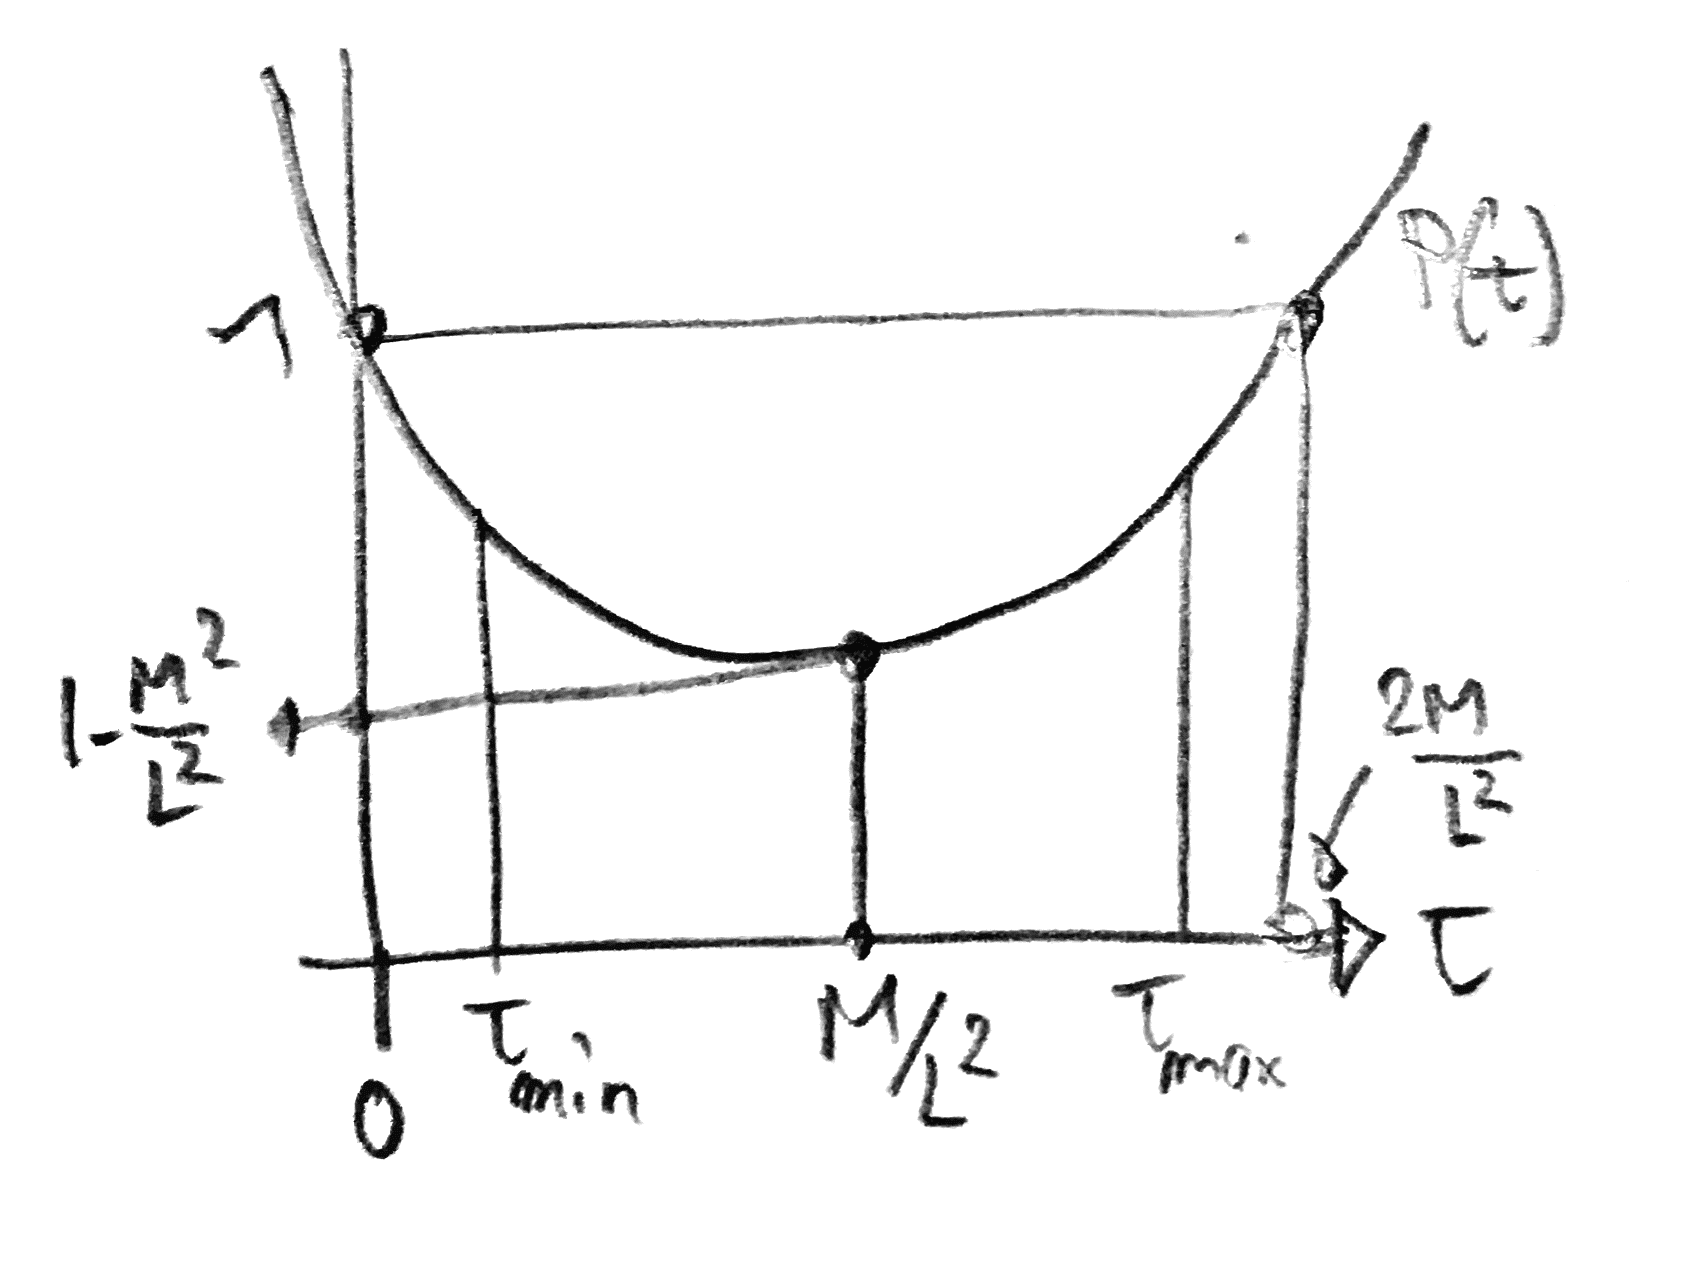
\includegraphics[width=.35\linewidth]{inverse-problems/grad-desc-general} \quad
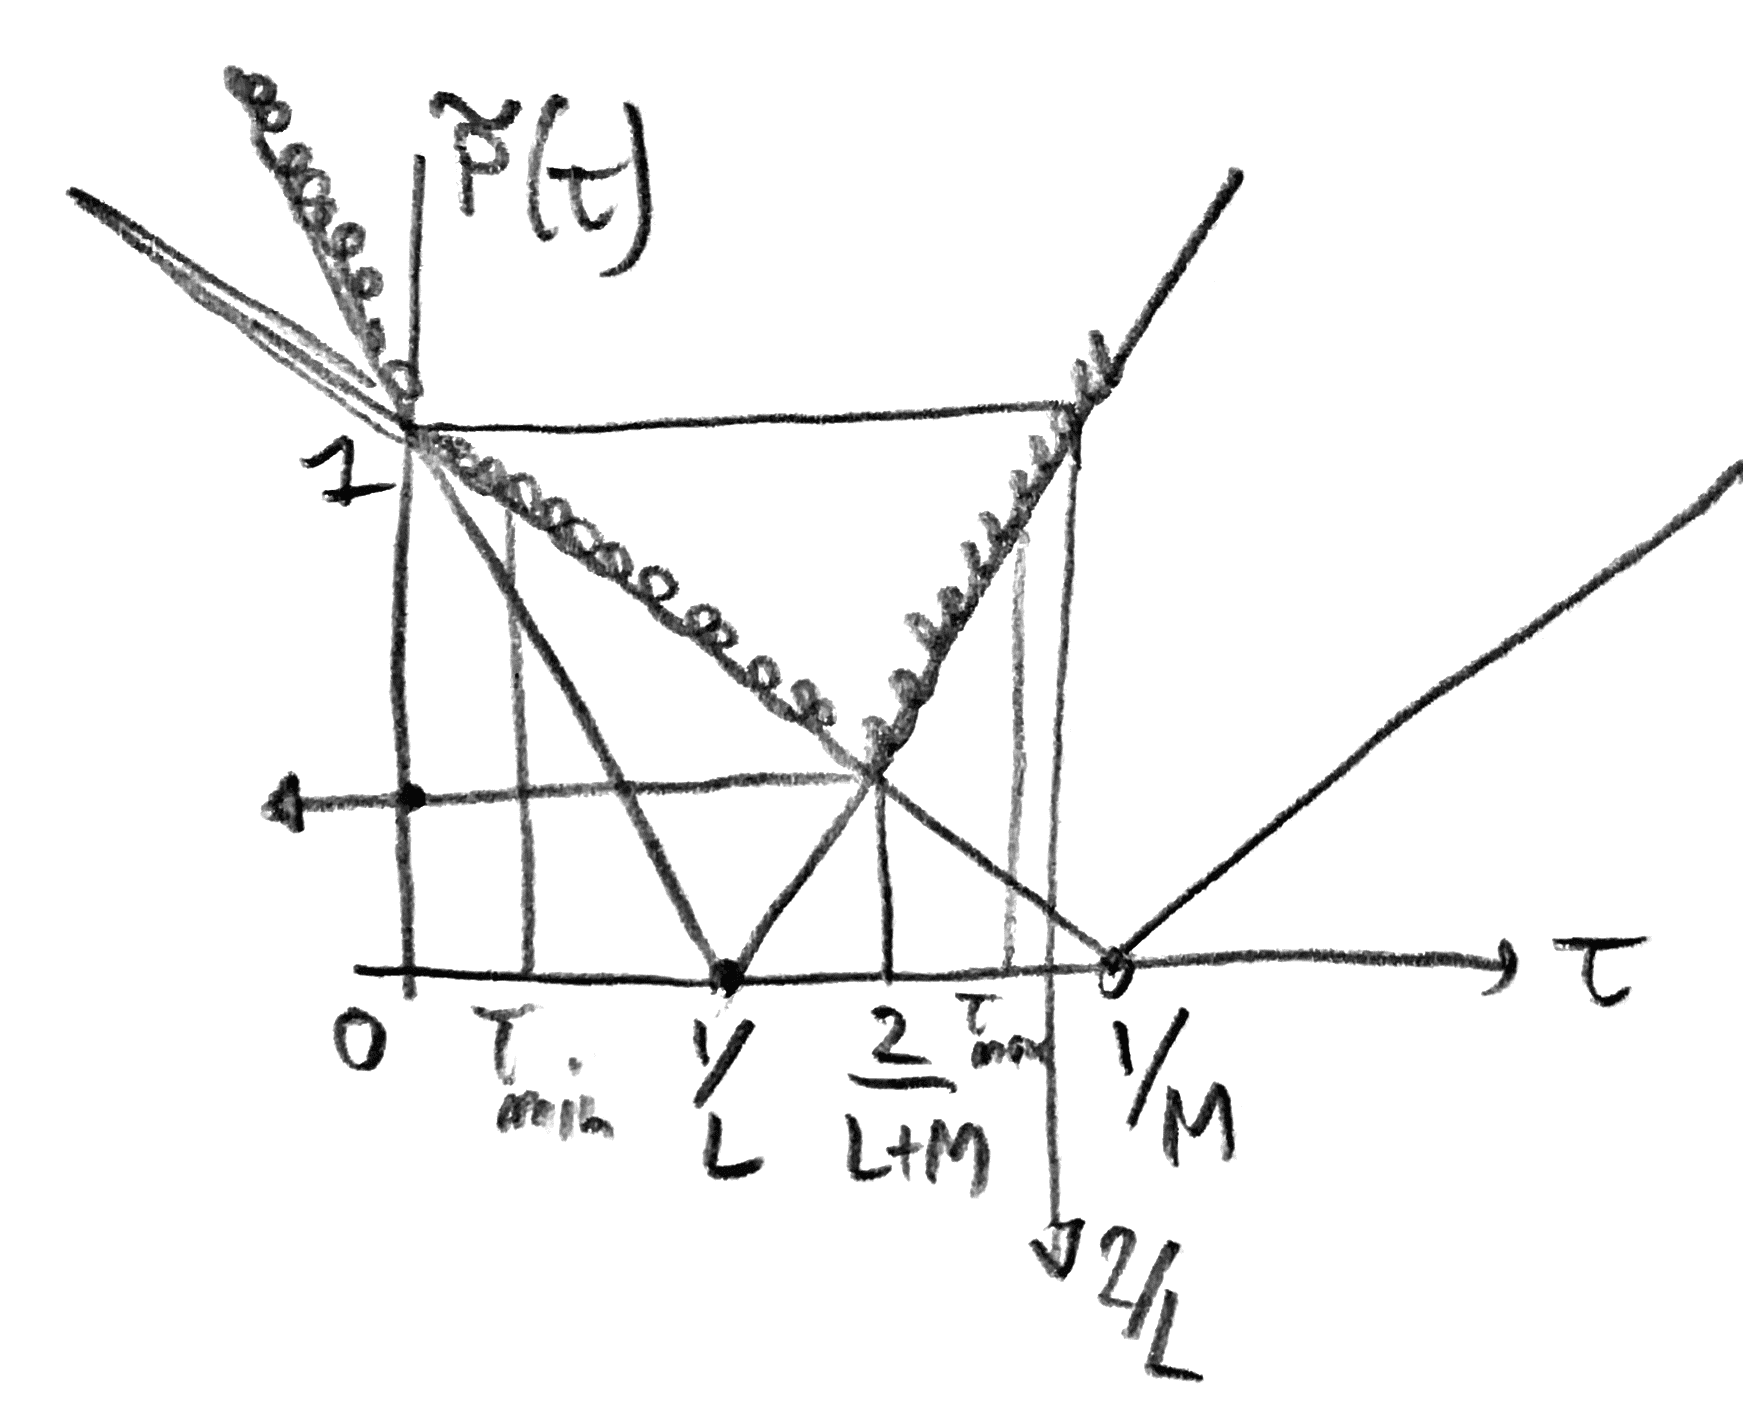
\includegraphics[width=.35\linewidth]{inverse-problems/grad-desc-linear}
\caption{\label{fig-grad-desc-contract}
Contraction constant $P(\tau)$ and $\tilde P(\tau)$ for a gradient descent step in the generic case (left) and for a quadratic function (right). 
}
\end{figure}


%

These two results are however complementary. Indeed, if the gradient descent converges, then ultimately $\it{x}$ is close to $x^\star$, so that one can approximate up to second order $f(x) \approx f(x^\star) + \dotp{Af}{f}-\dotp{f}{b}$ with $A=\partial^2 f(x^\star)$ and $b=-\nabla f(x^\star)$. So that the ``local'' rate, the one obtained after a large enough of iterations, is actually driven by $\tilde\rho$ and not $\rho$. It is thus important to distinguish between the global rate and the local rate. In practice, descent algorithm typically have two phase: a first ``slow'' phase govern by the global rate, and a second ``fast'' phase governed by the local rate. Unfortunately, the optimal step sizes $\tau_\ell$ are in general different for the two phase, so that optimal adaptation of step size is a difficult problems. This is why more advanced users typically use various line search strategies (to find the optimal step size at each iteration) or use second order information using quasi-Newton technics (BFGS).